%%%%%%%%%%%%%%%%%%%%%%%%%%%%%%%%%%%%%%%%%%%%%%%%%%%%%%%%%%%%%%%%%%%%%%
%%  Copyright by Wenliang Du                                 %%
%%  This work is licensed under the Creative Commons                %%
%%  Attribution-NonCommercial-ShareAlike 4.0 International License. %%
%%  To view a copy of this license, visit                           %%
%%  http://creativecommons.org/licenses/by-nc-sa/4.0/.              %%
%%%%%%%%%%%%%%%%%%%%%%%%%%%%%%%%%%%%%%%%%%%%%%%%%%%%%%%%%%%%%%%%%%%%%%

\newcommand{\commonfolder}{../../common-files}
\input{\commonfolder/header}
\input{\commonfolder/copyright}

\newcommand{\vpnFigs}{./Figs}

\lhead{\bfseries SEED Labs -- 虚拟专用网络实验:容器版本}

\begin{document}

\newcounter{task}
\setcounter{task}{1}
\newcommand{\mytask}{\bf {\noindent \arabic{task}} \addtocounter{task}{1} \,}



\begin{center}
{\LARGE 虚拟专用网络实验:容器版本}
\end{center}

\seedlabcopyright{2020}


% *******************************************
% SECTION
% ******************************************* 
\section{概述}

虚拟专用网络(VPN)是建立在公共网络(通常是因特网)之上的专用网络。
VPN内的计算机可以安全的进行通信,就像它们在一个真实的、物理上与外界隔离的专用网络上,
即使它们的流量会通过公共网络。
VPN使得员工们在旅行时可以安全的接入公司网络;它还允许公司将他们的专用网络扩展到全国各地乃至世界各地。


本实验的目标是帮助学生理解VPN的工作原理。
我们专注于一种特定类型的VPN(最常见的类型),它是建立在传输层之上。
我们将从头开始构建一个非常简单的VPN,并使用该过程来解释VPN技术的每个部分是如何工作的。
一个真正的VPN项目有两个基本部分,隧道和加密。本实验只关注隧道部分,帮助学生理解隧道技术,所以在这个实验中的隧道是没有被加密的。
还有另一个更加全面的VPN实验,其中包括加密部分。
本实验涵盖以下主题:

\begin{itemize}[noitemsep]
\item 虚拟专用网络
\item TUN/TAP虚拟接口
\item IP隧道
\item 路由
\end{itemize}


\paragraph{书籍和视频}
TUN/TAP虚拟接口的详细介绍以及VPN的工作原理可参见一下内容:

\begin{itemize}[noitemsep]
\item Chapter 19 of the SEED Book, \seedbook
\item Section 8 of the SEED Lecture, \seedisvideo
\end{itemize}


\paragraph{相关实验}
本实验仅涵盖VPN隧道部分,而完整的VPN还需要保护其隧道。
我们有一个另外单独的实验叫做VPN Lab,这是一个综合性的实验,包括隧道和保护部分。
学生可以先解决这个隧道实验。在学习了PKI和TLS之后,他们可以再进入这个综合性的VPN实验。


\paragraph{实验环境}
本实验已在SEED Ubuntu 20.04 VM上进行了测试。
您可以从SEED网站下载一个预构建的映像,然后在您自己的计算机上运行这个SEED VM。
但是,大部分SEED实验都可以在云端进行,您可以根据我们的说明在云端创建一个SEED虚拟机。


% *******************************************
% SECTION
% ******************************************* 
\section{Task 1: 网络设置}

我们将在计算机(客户端)和网关之间建立一条VPN隧道,允许计算机通过网关安全地访问专用网络。
我们需要至少3台机器:VPN客户端(也用作主机主机U)、VPN服务器(路由器/网关)和一台在专用网络中的主机(主机V)。
网络设置如图1所示。


\begin{figure}[htb]
  \begin{center}
    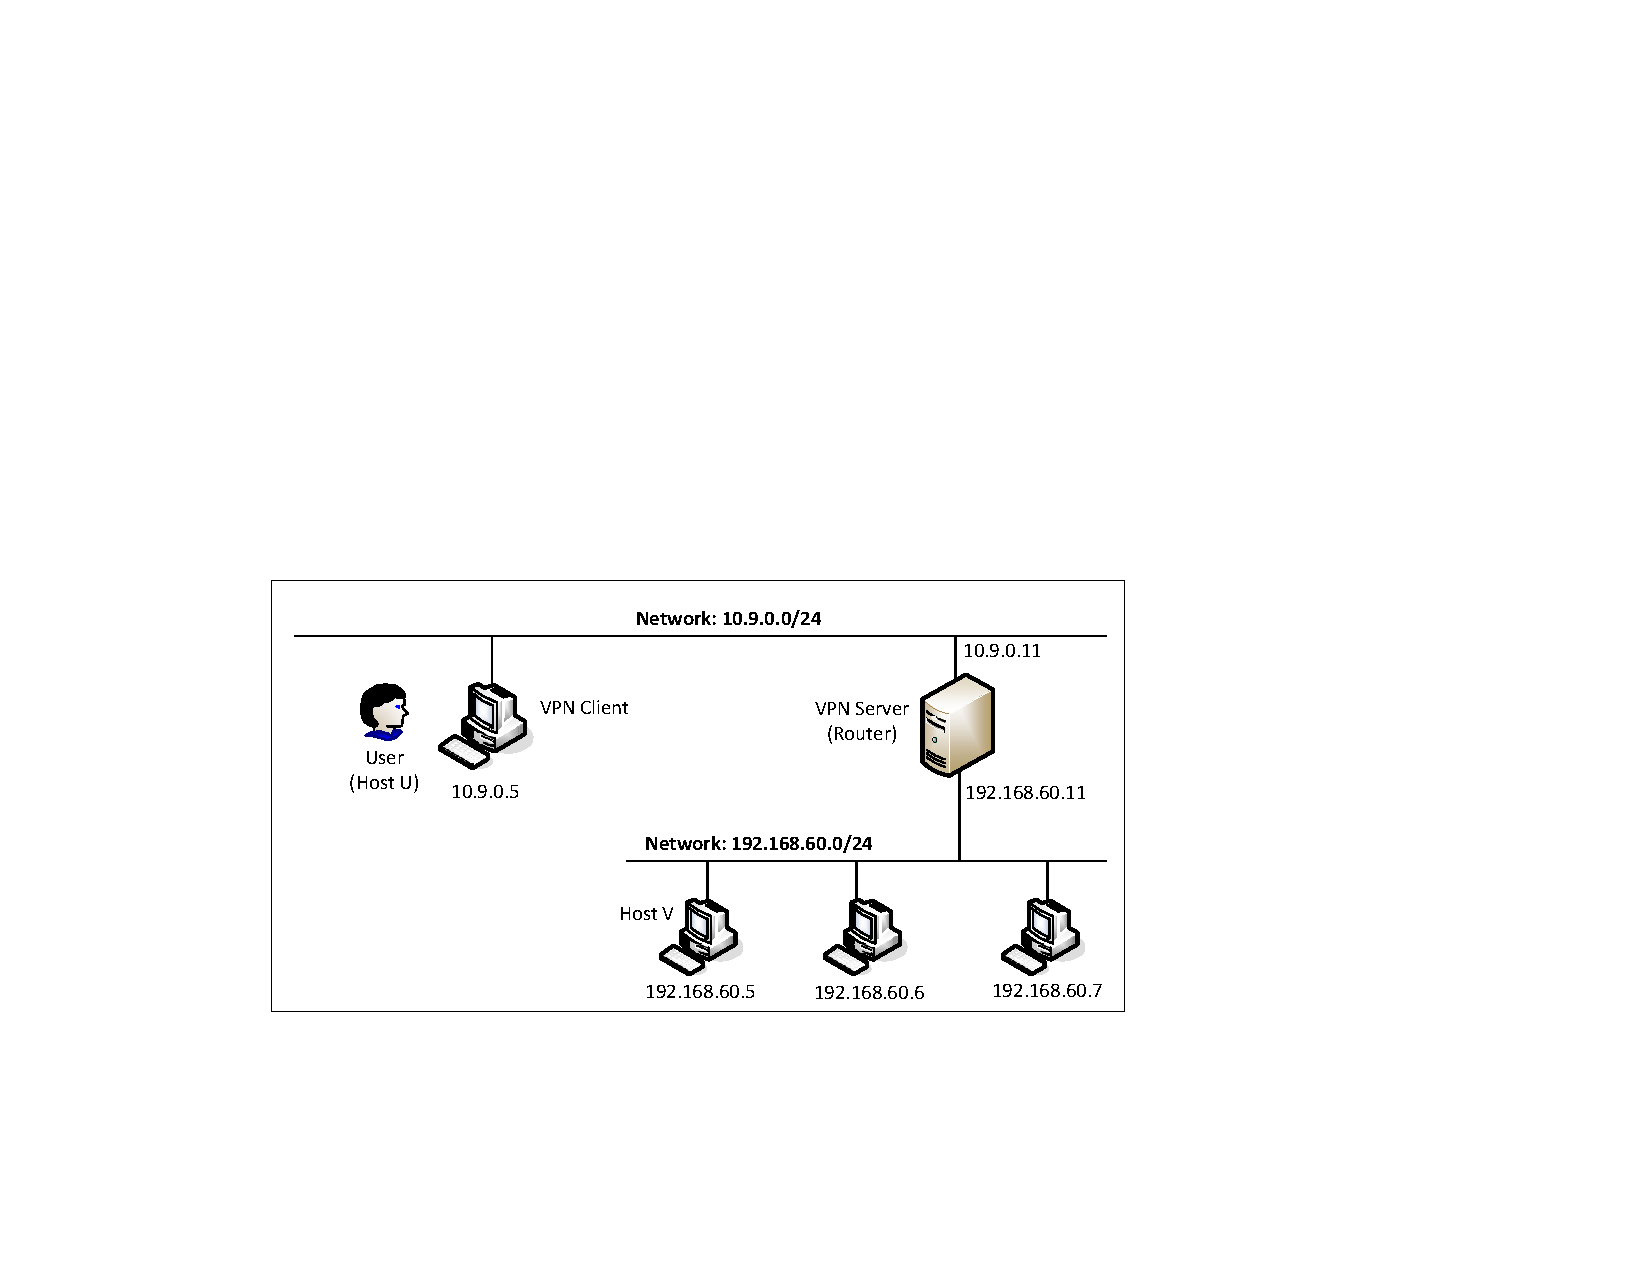
\includegraphics[width=0.9\textwidth]{\vpnFigs/VPN_2lans.pdf}
  \end{center}
  \caption{实验环境设置}
  \label{vpn:fig:labenv}
\end{figure}


实际上,VPN客户端和VPN服务端是通过因特网连接的。
为了简单起见,我们在这个实验直接将这两台机器连接到同一个局域网,即这个局域网模拟互联网。


第三台机器主机V是专用网络内的一台计算机。主机U上的用户(专用网络之外)希望通过VPN隧道与主机V通信。
为了模拟这个设置,我们将主机V连接到VPN服务器(也用作网关)。在这样的设置中,主机V不能直接从Internet访问;
也不能从主机U直接访问。


\paragraph{实验设置}
请从实验网站上下载Labsetup.zip文件到你的虚拟机,解压,
进入Labsetup文件夹并使用docker-compose.yml文件来设置实验环境。
该文件内容的详细解释以及所有涉及的Dockerfile都可以在用户手册中找到,该手册链接在本实验的网站上。
如果这是您第一次使用容器来设置SEED实验环境,那么阅读用户手册非常重要。


在下文中,我们列出了一些与Docker和Compose相关的常用命令。由于我们将非常频繁的使用这些命令,
因此我们在.bashrc文件中为它们创建了别名(在我们提供的SEEDUbuntu 20.04 VM中)。

\begin{lstlisting}
$ docker-compose build # Build the container image
$ docker-compose up # Start the container
$ docker-compose down # Shut down the container
// Aliases for the Compose commands above
$ dcbuild # Alias for: docker-compose build
$ dcup # Alias for: docker-compose up
$ dcdown # Alias for: docker-compose down
\end{lstlisting}

所有容器都将在后台运行。要在容器上运行命令,我们通常需要在该容器上获取shell。
我们首先需要使用“\verb|docker ps|”命令找出容器的ID,
然后使用“\verb|docker exec|”命令在该容器上启动一个shell。
我们在 .bashrc 文件中为它们创建了别名。

\begin{lstlisting}
$ dockps // Alias for: docker ps --format "{{.ID}} {{.Names}}"
$ docksh <id> // Alias for: docker exec -it <id> /bin/bash

// The following example shows how to get a shell inside hostC
$ dockps
b1004832e275 hostA-10.9.0.5
0af4ea7a3e2e hostB-10.9.0.6
9652715c8e0a hostC-10.9.0.7

$ docksh 96
root@9652715c8e0a:/#

// Note: If a docker command requires a container ID, you do not need to
//       type the entire ID string. Typing the first few characters will
//       be sufficient, as long as they are unique among all the containers.
\end{lstlisting}

如果您在设置实验环境时遇到问题,请阅读手册的“常见问题”部分以获取可能的解决方案。


\paragraph{共享文件夹}
在这个实验中,我们需要编写自己的代码并在容器中运行它。 
在VM中进行代码编辑比在容器中更方便,因为我们可以使用自己喜欢的编辑器。 
为了虚拟机和容器共享文件,我们使用Docker volumes在虚拟机和容器之间创建了一个共享文件夹。 
如果您查看Docker Compose文件,您会发现我们在一些容器中添加了以下条目。 
它表示将主机(即虚拟机)上的 \verb|./volumes|文件夹挂载到容器内的\verb|/volumes|文件夹中。 
我们将在(虚拟机上的)\verb|./volumes|文件夹中编写代码,以便在容器内使用它们。

\begin{lstlisting}
volumes:
       - ./volumes:/volumes
\end{lstlisting}


\paragraph{数据包嗅探}
能够嗅探数据包在本实验中非常重要,因为如果事情没有按预期进行,能够查看数据包的去向可以帮助我们识别问题。
有几种不同的方法可以进行数据包嗅探:

\begin{itemize}
\item 在容器上运行\verb|tcpdump|。我们已经在每个容器上安装了\verb|tcpdump|。 要嗅探通过特定接口的数据包,我们只需要找出接口名称,然后执行以下操作(假设接口名称为\verb|eth0|):

\begin{lstlisting}
# tcpdump -i eth0 -n
\end{lstlisting}

需要注意的是在容器内部,由于Docker创建的隔离,当我们在容器内部运行\verb|tcpdump|时,
我们只能嗅探进出这个容器的数据包。
我们将无法嗅探其他容器之间的数据包。 
但是,如果容器在其网络设置中使用\verb|host|模式,它可以嗅探其他容器的数据包。
\item 在虚拟机上运行\verb|tcpdump|。如果我们在VM上运行\verb|tcpdump|,
我们对容器没有限制,我们可以嗅探容器之间的所有数据包。VM上的网络接口名称与容器上的不同。
在容器上,每个接口名称通常以\verb|eth|开头; 
在VM上,Docker创建的网络的接口名称以\verb|br-|开头,后跟网络的ID。
您始终可以使用\verb|ip address|命令获取VM和容器上的接口名称。
\item 我们还可以在虚拟机上运行Wireshark来嗅探数据包。
与\verb|tcpdump|类似,我们需要选择我们希望Wireshark嗅探的接口。
\end{itemize}


\paragraph{测试}
请进行以下测试以确保实验环境设置正确:

\begin{itemize}[noitemsep]
\item Host U可以与VPN Server通信。
\item VPN Server可以与主机 V通信。 
\item 主机 U应该不能与主机 V通信。
\item 在路由器上运行\verb|tcpdump|,并嗅探每个网络上的流量。展示表明您可以捕获数据包。
\end{itemize}


% *******************************************
% SECTION
% *******************************************
\section{Task 2: 创建和配置TUN接口} 

我们将要构建的VPN隧道基于TUN/TAP技术。 
TUN和TAP是虚拟网络内核驱动程序;
他们实现了完全由软件支持的网络设备。 
TAP(如网络分路)模拟以太网设备,它使用第2层数据包(例如以太网帧)进行操作;
TUN(如在网络 TUNnel 中)模拟网络层设备,它使用第3层数据包(例如IP数据包)进行操作。
使用TUN/TAP,我们可以创建虚拟网络接口。

用户空间程序通常连接到TUN/TAP虚拟网络接口。
操作系统通过TUN/TAP网络接口发送的数据包被传递到用户空间程序。
另一方面,程序通过TUN/TAP网络接口发送的数据包被注入到操作系统网络堆栈。
对于操作系统来说,数据包似乎是来自一个通过虚拟网络接口的外部源。

当程序连接到TUN/TAP接口时,内核发送到该接口的IP数据包将通过管道传送到程序中。
另一方面,通过程序写入接口的IP数据包将通过管道进入内核,
就好像它们是通过这个虚拟网络接口从外部来的一样。
该程序可以使用标准的\verb|read()|和\verb|write()|系统调用从虚拟接口接收数据包或将数据包发送到虚拟接口。

本任务的目的是熟悉TUN/TAP技术。
我们将进行几次实验来了解TUN/TAP接口的技术细节。
我们将使用以下Python程序作为实验的基础,并在整个实验过程中修改此基础代码。
该代码已包含在zip文件的volumes文件夹中。

\begin{center}
Listing 1:创建TUN接口(tun.py)
\end{center}
\begin{lstlisting}
#!/usr/bin/env python3
import fcntl
import struct
import os
import time
from scapy.all import *

TUNSETIFF = 0x400454ca
IFF_TUN = 0x0001
IFF_TAP = 0x0002
IFF_NO_PI = 0x1000

# Create the tun interface
tun = os.open("/dev/net/tun", os.O_RDWR)
ifr = struct.pack(’16sH’, b’tun%d’, IFF_TUN | IFF_NO_PI)
ifname_bytes = fcntl.ioctl(tun, TUNSETIFF, ifr)

# Get the interface name
ifname = ifname_bytes.decode(’UTF-8’)[:16].strip("\x00")
print("Interface Name: {}".format(ifname))

while True:
    time.sleep(10)
\end{lstlisting}


% *******************************************
% SUBSECTION
% ******************************************* 
\subsection{Task 2.a: 接口名称}

我们将在主机U上运行\verb|tun.py|程序。使上述\verb|tun.py|程序可执行,并使用root权限运行它。 
请参阅以下命令:

\begin{lstlisting}
// Make the Python program executable
# chmod a+x tun.py

// Run the program using the root privilege
# tun.py
\end{lstlisting}

程序一旦执行,就会阻塞。 
您可以转到另一个终端并在容器上获得一个新的shell。 
然后打印出机器上的所有接口。 
请在运行以下命令后报告您的观察结果:

\begin{lstlisting}
# ip address
\end{lstlisting}

您应该能够找到一个名为\verb|tun0|的接口。 
您在此任务中的工作是更改\verb|tun.py|程序,
因此不要使用\verb|tun|作为接口名称的前缀,而是使用您的姓氏作为前缀。 
例如,如果您的姓氏是\verb|smith|,则应使用\verb|smith|作为前缀。 
如果您的姓氏很长,则可以使用前五个字符。 
请展示你的结果。

% *******************************************
% SUBSECTION
% ******************************************* 
\subsection{Task 2.b: 设置TUN接口}

此时,TUN接口是不可用的,因为它还没有被配置。 
在使用接口之前,我们需要做两件事。 
首先,我们需要为其分配一个IP地址。 
其次,我们需要调出接口,因为接口还处于down状态。 
我们可以使用以下两个命令进行配置:

\begin{lstlisting}
// Assign IP address to the interface
# ip addr add 192.168.53.99/24 dev tun0

// Bring up the interface
# ip link set dev tun0 up
\end{lstlisting}

为了方便起见,同学们可以在\verb|tun.py|中添加如下两行代码,
这样就可以由程序自动进行配置了。

\begin{lstlisting}
os.system("ip addr add 192.168.53.99/24 dev {}".format(ifname))
os.system("ip link set dev {} up".format(ifname))
\end{lstlisting}

运行上面两个命令后,再次运行“\verb|ip address|”命令,报告你的观察结果。
与运行配置命令之前的情况有何不同?

% *******************************************
% SUBSECTION
% ******************************************* 
\subsection{Task 2.c: 从TUN接口读取}

在此任务中,我们将从TUN接口读取。 
从TUN接口发出的任何内容都是IP数据包。 
我们可以将从接口接收到的数据转换成一个Scapy IP对象,
这样我们就可以打印出IP数据包的每个字段。 
请使用以下\verb|while|循环替换\verb|tun.py|中的循环:

\begin{lstlisting}
while True:
  # Get a packet from the tun interface
  packet = os.read(tun, 2048)
  if packet:
    ip = IP(packet)
    print(ip.summary())
\end{lstlisting}

请在主机U上运行修改后的\verb|tun.py|程序,并相应配置TUN接口,然后进行以下实验。 
请描述您的观察:

\begin{itemize}
\item 在主机U上,\verb|ping 192.168.53.0/24|网络中的主机。\verb|tun.py|程序打印出什么?
发生了什么事?为什么?
\item 在主机U上,\verb|ping|内部网络\verb|192.168.60.0/24|中的主机,
\verb|tun.py|是否打印出任何内容?为什么?
\end{itemize}

% *******************************************
% SUBSECTION
% ******************************************* 
\subsection{Task 2.d: 写入TUN接口}

在这个任务中,我们将写入TUN接口。 
由于这是一个虚拟网络接口,因此应用程序写入该接口的任何内容都将以IP数据包的形式出现在内核中。

我们将修改\verb|tun.py|程序,所以在从TUN接口得到一个数据包后,
我们根据收到的数据包构造一个新的数据包。 
然后我们将新数据包写入TUN接口。 
如何构建新数据包取决于学生。 
以下代码显示了如何将一个IP数据包写入TUN接口的示例。

\begin{lstlisting}
# Send out a spoof packet using the tun interface
newip = IP(src=’1.2.3.4’, dst=ip.src)
newpkt = newip/ip.payload
os.write(tun, bytes(newpkt))
\end{lstlisting}

请根据以下要求修改\verb|tun.py|代码:

\begin{itemize}
\item 从TUN接口得到一个报文后,如果这个报文是\verb|ICMP echo request|报文,
则构造一个对应的\verb|echo reply|报文写入TUN接口。 
请提供证据证明代码按预期工作。
\item 不要将IP数据包写入接口,而是将一些任意数据写入接口,并报告您的观察结果。
\end{itemize}


% *******************************************
% SECTION
% *******************************************
\section{Task 3: 通过隧道将IP数据包发送到VPN服务器} 

在这个任务中,我们将从TUN接口接收到的IP数据包放入新IP数据包的UDP有效负载字段中,
并将其发送到另一台计算机。 
也就是说,我们将原始数据包放入一个新数据包中。 
这称为IP隧道。 
隧道的实现只是标准的客户端/服务器编程。 
它可以构建在TCP或UDP之上。 
在此任务中,我们将使用UDP。 
即我们将IP数据包放入UDP数据包的有效负载字段中。

\paragraph{服务器程序tun\_server.py} 
我们将在VPN Server上运行\verb|tun_server.py|程序。
这个程序只是一个标准的UDP服务器程序。 
它监听端口9090并打印出接收到的任何内容。
程序假设UDP有效负载字段中的数据是一个IP数据包,
因此它将有效负载转换为Scapy IP对象,并打印出这个封闭的IP数据包的源IP地址和目标IP地址。

\begin{center}
Listing 2:tun\_server.py
\end{center}
\begin{lstlisting}
#!/usr/bin/env python3

from scapy.all import *

IP_A = "0.0.0.0"
PORT = 9090

sock = socket.socket(socket.AF_INET, socket.SOCK_DGRAM)
sock.bind((IP_A, PORT))

while True:
  data, (ip, port) = sock.recvfrom(2048)
  print("{}:{} --> {}:{}".format(ip, port, IP_A, PORT))
  pkt = IP(data)
  print(" Inside: {} --> {}".format(pkt.src, pkt.dst))
\end{lstlisting}


\paragraph{实现客户端程序tun\_client.py} 
首先,我们需要修改TUN程序\verb|tun.py|。 
让我们重命名它,并将其命名为\verb|tun_client.py|。 
使用标准套接字编程可以使用UDP向另一台计算机发送数据。 

将程序中的\verb|while|循环替换为以下内容: 
SERVER IP 和 SERVER PORT 应替换为VPN Server上运行的服务器程序的实际IP地址和端口号。

\begin{lstlisting}
# Create UDP socket
sock = socket.socket(socket.AF_INET, socket.SOCK_DGRAM)

while True:
  # Get a packet from the tun interface
  packet = os.read(tun, 2048)
  if packet:
    # Send the packet via the tunnel
    sock.sendto(packet, (SERVER_IP, SERVER_PORT))
\end{lstlisting}

\paragraph{测试}
在VPN Server上运行\verb|tun_server.py|程序,
然后在主机U上运行\verb|tun_client.py|。
要测试隧道是否工作,
请ping任何属于192.168.53.0/24网络的IP地址。 
VPN Server上打印的内容是什么?为什么? 

我们的最终目标是使用隧道访问私有网络192.168.60.0/24内的主机。 
让我们ping主机V,看看ICMP数据包是否通过隧道发送到VPN Server。 
如果没有,有什么问题? 
你需要解决这个问题,这样才能通过隧道发送ping数据包。 
这是通过路由完成的,即去往192.168.60.0/24网络的数据包应该被路由到TUN接口并被交给\verb|tun_client.py|
程序。 
以下命令显示如何将条目添加到路由表:

\begin{lstlisting}
# ip route add <network> dev <interface> via <router ip>
\end{lstlisting}

请提供证据证明您在ping一个在192.168.60.0/24网络中的IP地址时,
通过隧道\verb|tun_server.py|接收到了ICMP数据包。


% *******************************************
% SECTION
% *******************************************
\section{Task 4: 设置VPN服务器} 

在\verb|tun_server.py|从隧道中获取数据包后,它需要将数据包提供给内核,
以便内核可以将数据包路由到其最终目的地。
这需要通过一个TUN接口来完成,就像我们在任务2中所做的一样。
请修改\verb|tun_server.py|,使其可以执行以下操作:

\begin{itemize}
\item 创建一个TUN接口并对其进行配置。
\item 从套接字接口获取数据;将接收到的数据视为IP数据包。
\item 将数据包写入TUN接口。
\end{itemize}

在运行修改后的\verb|tun_server.py|之前,我们需要启用IP转发。
除非特别配置,否则计算机将仅充当主机,而不充当网关。 
VPN服务器需要在私网和隧道之间转发数据包,所以需要起到网关的作用。
我们需要为计算机启用IP转发,使其表现得像网关。
路由器容器上已启用IP转发。
您可以在docker-compose.yml中看到路由器容器具有以下条目:

\begin{lstlisting}
sysctls:
        - net.ipv4.ip_forward=1
\end{lstlisting}

\paragraph{测试} 如果一切设置正确,我们可以从主机U\verb|ping|主机V。
ICMP回显请求数据包最终应该通过隧道到达主机V。 
请展示你的验证证明。 
需要注意的是,虽然主机V会响应ICMP数据包,
但回复不会回到主机U,因为我们还没有设置好一切。 
因此,对于此任务,显示(使用Wireshark或tcpdump)ICMP数据包已到达主机V就足够了。

% *******************************************
% SECTION
% *******************************************
\section{Task 5: 处理双向流量} 

到此之后,你的隧道的一个方向就完成了,即我们可以通过隧道将数据包从主机U发送到主机V。
如果我们查看主机V上的Wireshark跟踪,我们可以看到主机V已发出响应,但数据包在某处被丢弃。
这是因为我们的隧道只有一个方向;
我们需要设置它的另一个方向,因此返回的流量可以通过隧道返回到主机U。

为此,我们的TUN客户端和服务器程序需要从两个接口读取数据,
即TUN接口和套接字接口。
所有这些接口都由文件描述符表示,
所以我们需要监视它们以查看是否有来自它们的数据。
一种方法是不断轮询它们,并查看每个接口上是否有数据。
这种方法的性能是不可取的,因为当没有数据时,进程必须保持在空闲循环中运行。
另一种方法是从接口读取。默认情况下,读是阻塞的,即如果没有数据,进程将被挂起。
当数据可用时,进程将被解除阻塞,并继续执行。
这样就不会在没有数据的时候浪费CPU时间。

基于读取的阻塞机制适用于一个接口。
如果一个进程在多个接口上等待,它不能只在其中一个接口上阻塞。
它必须在所有接口上一起阻塞。 
Linux有一个称为select()的系统调用,它允许程序同时监视多个文件描述符。
要使用select(),我们需要将所有要监视的文件描述符存储在一个集合中,
然后我们将该集合提供给select()系统调用,它将阻塞该进程,直到集合中的一个文件描述符上的数据可用。
我们可以检查哪个文件描述符接收到了数据。
在下面的Python代码片段中,我们使用select()来监控TUN和套接字文件描述符。

\begin{lstlisting}
# We assume that sock and tun file descriptors have already been created.

while True:
  # this will block until at least one interface is ready
  ready, _, _ = select.select([sock, tun], [], [])

  for fd in ready:
    if fd is sock:
      data, (ip, port) = sock.recvfrom(2048)
      pkt = IP(data)
      print("From socket <==: {} --> {}".format(pkt.src, pkt.dst))
      ... (code needs to be added by students) ...

    if fd is tun:
      packet = os.read(tun, 2048)
      pkt = IP(packet)
      print("From tun ==>: {} --> {}".format(pkt.src, pkt.dst))
      ... (code needs to be added by students) ...
\end{lstlisting}

同学们可以用上面的代码替换TUN客户端和服务端程序中的while循环。代码不完整;学生应该完成它。

\paragraph{测试} 完成此操作后,我们应该能够从机器U与机器V通信,并且VPN隧道(未加密)现在已完成。
请使用有关ping和telnet命令显示您的wireshark验证。 
在你的证明中,你需要指出你的数据包是如何流动的。


% *******************************************
% SECTION
% *******************************************
\section{Task 6: 隧道突破实验} 

在主机U上,远程登录到主机V。
在保持telnet连接处于活动状态的同时,
我们通过停止\verb|tun_client.py|或\verb|tun_server.py|程序来破坏VPN隧道。 
然后我们在telnet窗口中输入一些内容。 
你看到你输入的内容了吗?TCP连接会发生什么?连接是否断开? 

现在让我们重新连接VPN隧道(不要等待太久)。 
我们将再次运行\verb|tun_client.py|和\verb|tun_server.py|程序,
并设置它们的TUN接口和路由(在这里您可以发现在程序中包含配置命令将使您的生活更轻松)。
一旦隧道重新建立,telnet连接会发生什么? 
请描述并解释您的观察结果。


% *******************************************
% SECTION
% *******************************************
\section{Task 7: 主机V上的路由实验} 

在真实的VPN系统中,流量会被加密(本实验不涉及这部分)。
这意味着返回流量必须从同一隧道返回。
如何获取从主机V到VPN服务器的返回流量并非易事。
我们的设置简化了这种情况。
在我们的设置中,主机V的路由表有一个默认设置:
去往任何目的地的数据包,除了192.168.60.0/24网络,将被自动路由到VPN服务器。

在现实世界中,主机V可能距离VPN服务器只有几跳,
默认路由条目可能无法保证将返回的数据包路由回VPN服务器。
必须正确设置专用网络内的路由表,以确保将到达隧道另一端的数据包路由到VPN服务器。
为了模拟这种情况,我们将从主机V中删除默认条目,
并在路由表中添加更具体的条目,以便可以将返回的数据包路由回VPN服务器。
学生可以使用以下命令删除默认条目并添加新条目:

\begin{lstlisting}
// Delete the default entry
# ip route del default

// Add an entry
# ip route add <network prefix> via <router ip>
\end{lstlisting}


% *******************************************
% SECTION
% *******************************************
\section{Task 8: 专用网络之间的VPN} 

在此任务中,我们将在两个专用网络之间建立VPN。 
设置如图2所示。
整个设置在docker-compose2.yml文件中进行了描述,
您可以使用“\verb|-f docker-compose2.yml|”选项让docker-compose使用该文件,
而不是默认的docker-compose.yml文件。

\begin{figure}[htb]
  \begin{center}
    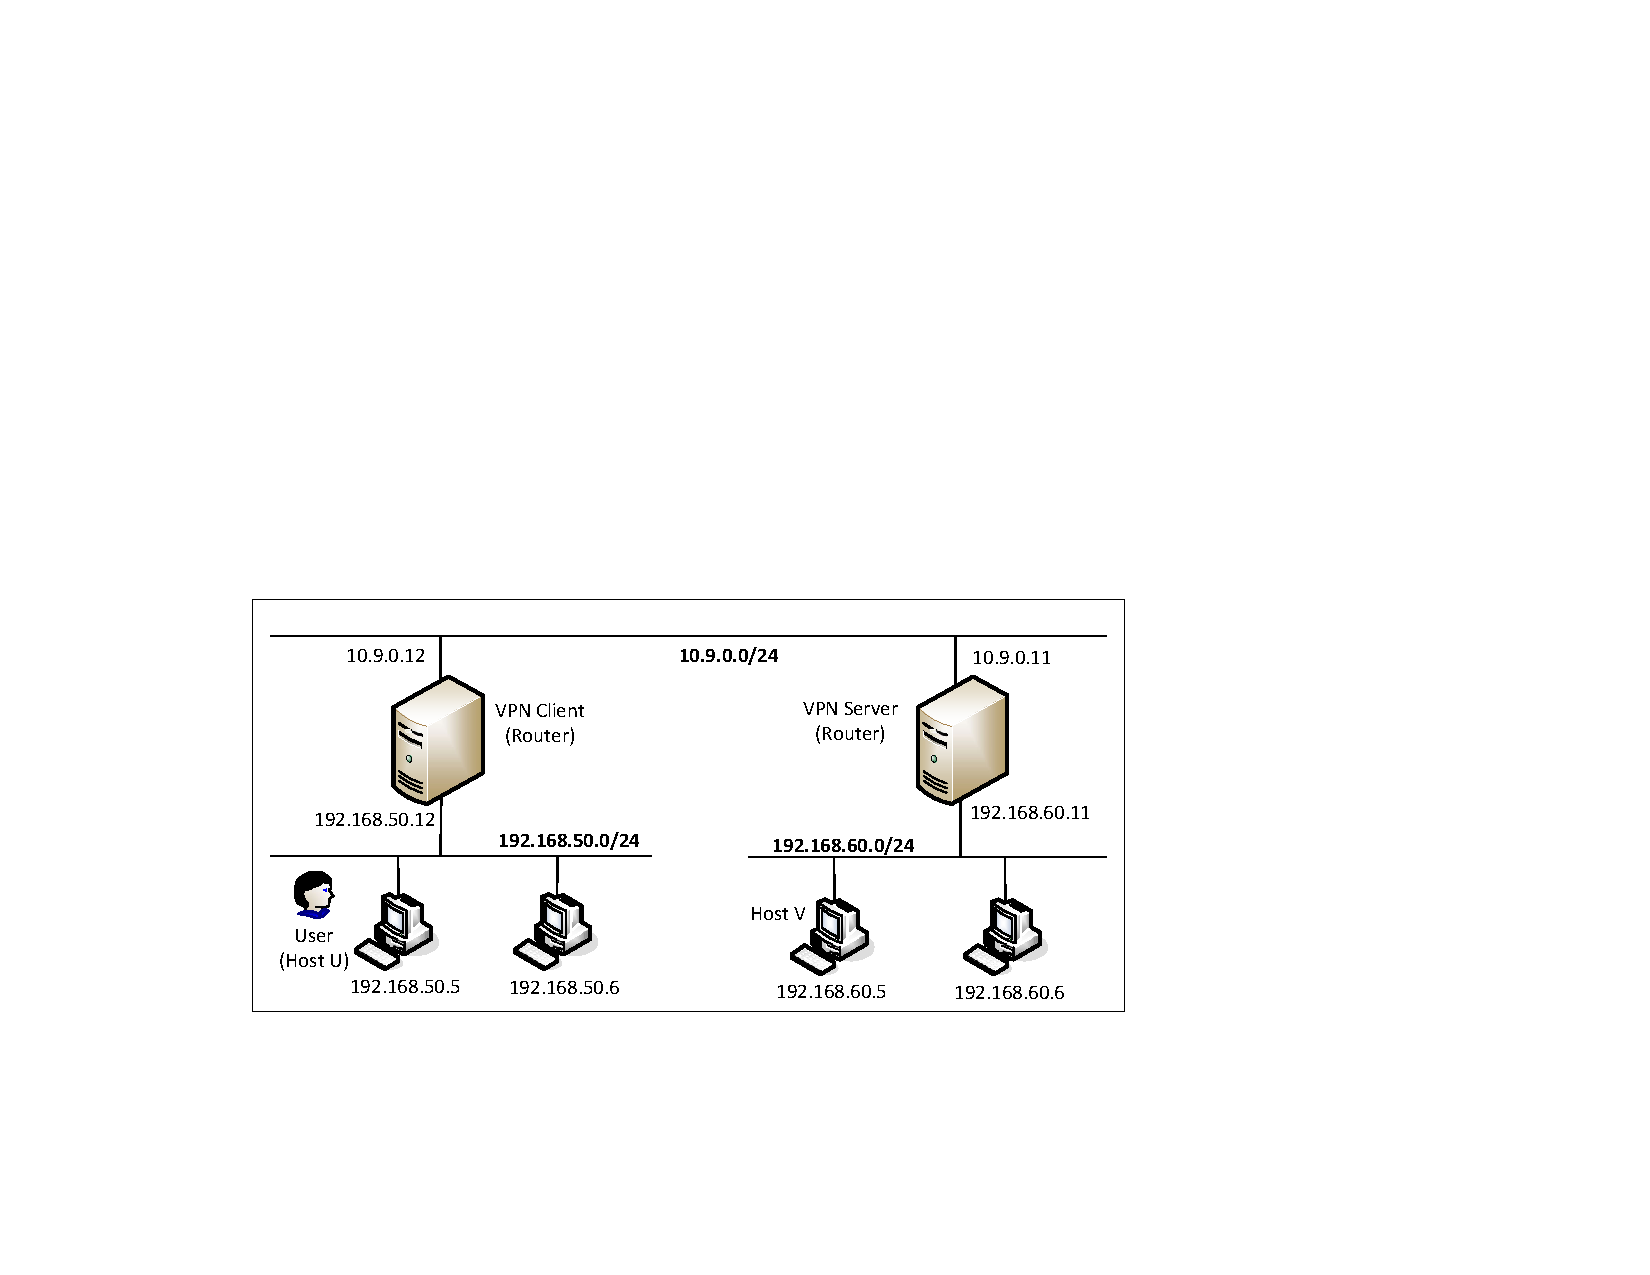
\includegraphics[width=0.9\textwidth]{\vpnFigs/VPN_3lans.pdf}
  \end{center}
  \caption{两个专用网络之间的VPN}
  \label{vpn:fig:vpn-2pn}
\end{figure}

\begin{lstlisting}
$ docker-compose -f docker-compose2.yml build
$ docker-compose -f docker-compose2.yml up
$ docker-compose -f docker-compose2.yml down
\end{lstlisting}

此设置模拟了一个组织有两个站点的情况,每个站点都有一个专用网络。 
连接这两个网络的唯一方法是通过Internet。 
您的任务是在这两个站点之间建立VPN,因此这两个网络之间的通信将通过VPN隧道。 
您可以使用之前开发的代码,但您需要考虑如何设置正确的路由,
以便这两个专用网络之间的数据包可以路由到VPN隧道。 
在你的报告中,请描述并解释你做了什么。 
您需要提供证据证明两个专用网络之间的数据包确实通过VPN隧道。


% *******************************************
% SECTION
% *******************************************
\section{Task 9: 用TAP接口实验} 

在这个任务中,我们将用TAP接口做一个简单的实验,让学生对这种类型的接口有所了解。 
TAP接口的工作方式与TUN接口非常相似。
主要区别在于TUN接口的内核端挂接到IP层,而TAP接口的内核端挂接到MAC层。
因此,通过TAP接口的报文包含MAC头,而通过TUN接口的报文只包含IP头。
除了获取包含IP数据包的帧外,应用程序还可以使用TAP接口获取其他类型的帧,例如ARP帧。

我们将使用以下程序进行实验,并且我们将只使用VPN客户端容器(实验室环境设置都可以)。
创建TUN接口和TAP接口的代码是相当相似的;
唯一的区别在于接口类型。
对于TAP接口,我们使用\verb|IFF_TAP|,而对于TUN,我们使用\verb|IFF_TUN|。
其余代码相同,以下不再赘述。 
TAP接口的配置方法与TUN接口的配置方法完全相同。

\begin{lstlisting}
...
tap = os.open("/dev/net/tun", os.O_RDWR)
ifr = struct.pack(’16sH’, b’tap%d’, IFF TAP | IFF_NO_PI)
ifname_bytes = fcntl.ioctl(tap, TUNSETIFF, ifr)
ifname = ifname_bytes.decode(’UTF-8’)[:16].strip("\x00")
...

while True:
  packet = os.read(tap, 2048)
  if packet:
    ether = Ether(packet)
    print(ether.summary())
\end{lstlisting}

上面的代码只是从TAP接口读取。 
然后它将数据转换为Scapy Ether对象,并打印出其所有字段。 
尝试在192.168.53.0/24网络中ping一个IP地址; 
报告并解释你的观察。

为了让这个更有趣,一旦你从TAP接口得到一个以太网帧,你可以检查它是否是一个ARP请求; 
如果是,则生成相应的ARP回复并将其写入TAP接口。
下面提供了一个示例代码:

\begin{lstlisting}
while True:
  packet = os.read(tun, 2048)
  if packet:
    print("--------------------------------")
    ether = Ether(packet)
    print(ether.summary())

    # Send a spoofed ARP response
    FAKE_MAC = "aa:bb:cc:dd:ee:ff"
    if ARP in ether and ether[ARP].op == 1 :
      arp = ether[ARP]
      newether = Ether(dst=ether.src, src=FAKE_MAC)
      newarp = ARP(psrc=arp.pdst, hwsrc=FAKE_MAC, pdst=arp.psrc, hwdst=ether.src, op=2)
      newpkt = newether/newarp
      print("***** Fake response: {}".format(newpkt.summary()))
      os.write(tun, bytes(newpkt))
\end{lstlisting}

要测试您的TAP程序,您可以在任何IP地址上运行\verb|arping|命令。 
该命令通过指定的接口向指定的IP地址发出ARP请求。 
如果您的模仿arp回复(spoof-arp-reply)TAP程序有效,您应该能够得到响应。 
请参阅以下示例。

\begin{lstlisting}
arping -I tap0 192.168.53.33
arping -I tap0 1.2.3.4
\end{lstlisting}


% *******************************************
% SECTION
% ******************************************* 
\section{提交}

您需要提交一份详细的实验报告和屏幕截图,以描述您所做的和观察到的。 
您还需要对有趣或令人惊讶的观察结果提供解释。 
还请列出重要的代码片段并附上解释。 
简单地附上代码而没有任何解释将不会获得学分。


\end{document}



